\documentclass[a4paper,11pt]{article}
\input{/home/tof/Documents/Cozy/latex-include/preambule_doc.tex}
\input{/home/tof/Documents/Cozy/latex-include/preambule_commun.tex}
\newcommand{\showprof}{show them}  % comment this line if you don't want to see todo environment
\setlength{\fboxrule}{0.8pt}
\fancyhead[L]{\fbox{\Large{\textbf{Secu 03}}}}
\fancyhead[C]{\textbf{Chiffrement asymétrique - RSA}}
\newdate{madate}{10}{09}{2020}
%\fancyhead[R]{\displaydate{madate}} %\today
%\fancyhead[R]{Seconde - SNT}
%\fancyhead[R]{Première - NSI}
\fancyhead[R]{Terminale - NSI}
\fancyfoot[L]{\vspace{1mm}Christophe Viroulaud}
\AtEndDocument{\label{lastpage}}
\fancyfoot[C]{\textbf{Page \thepage/\pageref{lastpage}}}
\fancyfoot[R]{\includegraphics[width=2cm,align=t]{/home/tof/Documents/Cozy/latex-include/cc.png}}
\usepackage{tikz}

\begin{document}
\section{Problématique} 
Le chiffrement asymétrique de Diffie-Hellman permet d'échanger des clés via un canal non sûr mais ne gère pas les problèmes liés à l'authentification des interlocuteurs. En s'inspirant de ces travaux, \emph{Ron Rivest, Adi Shamir et Len Adleman} créent une méthode qui lève cette difficulté.
\begin{center}
    \framebox{Comment authentifier avec certitude les participants?}
\end{center}
\section{Chiffrement RSA}
\subsection{Principe}
%breveté en 1983 par MIT; expiration brevet en 2000
Les trois cryptologues décrivent leur algorithme en 1977. Tout comme Diffie et Hellman, ils s'appuient sur des \emph{fonctions à sens unique} et une paire de clés publique et privée.
\begin{aretenir}[]
    {\Large$$K_{priv}(K_{pub}(m))=K_{pub}(K_{priv}(m))=m$$}
\end{aretenir}
\newcommand{\puzzle}[3]{
    \draw[fill=white] (#1-0.6,#2) -- (#1-0.6,0.7+#2) -- (1+#1,0.7+#2) arc (220:-40:0.3) -- (3.1+#1,0.7+#2) -- (3.1+#1,#2) -- cycle;
    \node at(#1+1.25,0.35+#2){#3};
    }
\newcommand{\puzzlebis}[3]{
    \draw (#1-0.6,1.9+#2) -- (#1-0.6,0.7+#2) -- (1+#1,0.7+#2) arc (220:-40:0.3) -- (3.1+#1,0.7+#2) -- (3.1+#1,1.9+#2) -- cycle;
    \node at(#1+1.25,1.55+#2){#3};
    }
\begin{center}
    \begin{tikzpicture}[scale=0.9, transform shape]
        
        \node at(-4,0){Alice};
        \node at(0,0){Canal non sécurisé};
        \node at(4,0){Bob};
        \draw[dashed] (-2,0) -- (-2,-15) ;
        \draw[dashed] (2,0) -- (2,-15) ;

        \node[draw] at(0,-1){Étape 1};
        \puzzle{-5.2}{-3.2}{Clé publique};
        \puzzlebis{-5.2}{-3.2}{Clé privée};
        \node at(4,-2.5){Message};


        \node[draw] at(0,-4){Étape 2};
        \draw[->,>=latex] (-4,-5.8) -- (4,-5.8);
        \puzzle{0}{-6.2}{Clé publique};
        \puzzlebis{-5.2}{-6.2}{Clé privée};
        \node at(4,-5.5){Message};

        \node[draw] at(0,-7){Étape 3};
        \puzzle{3}{-9.2}{C\textbf{M}l\textbf{e}é \textbf{s}p\textbf{s}u\textbf{a}b\textbf{g}l\textbf{e}ique};
        \puzzlebis{-5.2}{-9.2}{Clé privée};

        \node[draw] at(0,-10){Étape 4};
        \draw[<-,>=latex] (-4,-11.8) -- (4,-11.8);
        \puzzle{-2}{-12.2}{C\textbf{M}l\textbf{e}é \textbf{s}p\textbf{s}u\textbf{a}b\textbf{g}l\textbf{e}ique};
        \puzzlebis{-5.2}{-12.2}{Clé privée};

        \node[draw] at(0,-13){Étape 5};
        \puzzle{-5.2}{-15.2}{Message};
        \puzzlebis{-5.2}{-15.2}{};

    \end{tikzpicture}
    \captionof{figure}{Clé publique / clé privée}
\end{center}
% Bob crée ses propres clés
Mathématiquement, la fonction respecte les règles suivantes:
\begin{itemize}
    \item Il est impossible de deviner la clé privée en connaissant la clé publique.
    \item Il est impossible de deviner le message avec une seule des deux clés.
\end{itemize}
\subsection{kid RSA: formalisme mathématique}
La création des clés suit un algorithme mathématique complexe. L'université de Rhode Island a produit une version simplifiée (à utilisation pédagogique) pour simuler le protocole.
\begin{activite}
\begin{enumerate}
    \item Découvrir l'algorithme \emph{kidrsa} sur la page \url{https://tinyurl.com/rsakid}
    \item Écrire la fonction \textbf{\texttt{creer\_nombre(a: int, b: int, a1: int, b1: int) $\rightarrow$ dict}} qui renvoie un dictionnaire contenant les clés privée et publique. Chaque clé sera un tuple.
    \item Écrire la fonction \textbf{\texttt{chiffrer(message: int, publique: tuple) $\rightarrow$ int}} qui encode \emph{message} avec la clé publique (\emph{e, n}).
    \item Écrire la fonction \textbf{\texttt{dechiffrer(message\_chiffre: int, privee: int) $\rightarrow$ int}} qui déchiffre \emph{message\_chiffre} avec la clé privée \emph{(d, n)}.
    \item Tester l'algorithme de chiffrage avec un entier (inférieur à n).
\end{enumerate}
\end{activite}

% toujours pas réglé le pb de l'authentification
\section{Authentification des participants}
Contrairement à la méthode de Diffie-Hellman, le protocole RSA peut être utilisé pour authentifier les participants. Il faut pour cela qu'un \textbf{tiers de confiance} (Nestor) intervienne.
\newcommand{\puzzlefill}[3]{
    \fill (#1-0.6,1.9+#2) -- (#1-0.6,0.7+#2) -- (1+#1,0.7+#2) arc (220:-40:0.3) -- (3.1+#1,0.7+#2) -- (3.1+#1,1.9+#2) -- cycle;
    \node at(#1+1.25,1.55+#2){#3};
    }
\begin{center}
    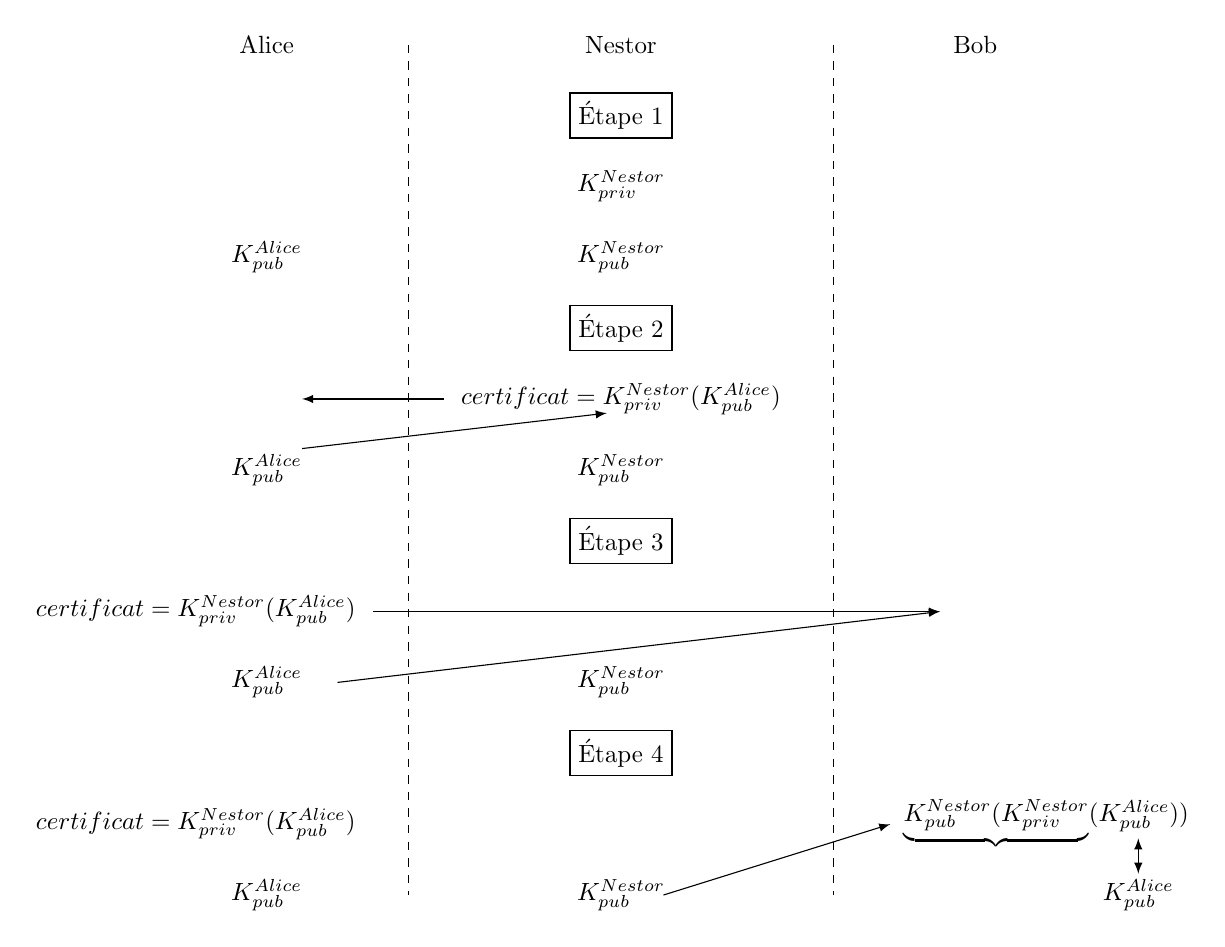
\begin{tikzpicture}[scale=0.9, transform shape]
        
        \node at(-5,0){Alice};
        \node at(0,0){Nestor};
        \node at(5,0){Bob};
        \draw[dashed] (-3,0) -- (-3,-12) ;
        \draw[dashed] (3,0) -- (3,-12) ;

        \node[draw] at(0,-1){Étape 1};
        \node at(-5,-3){$K^{Alice}_{pub}$};
        \node at(0,-2){$K^{Nestor}_{priv}$};
        \node at(0,-3){$K^{Nestor}_{pub}$};

        \node[draw] at(0,-4){Étape 2};
        \draw[<-,>=latex] (-4.5,-5) -- (-2.5,-5);
        \draw[->,>=latex] (-4.5,-5.7) -- (-0.2,-5.2);

        \node at(-5,-6){$K^{Alice}_{pub}$};
        \node at(0,-5){$certificat=K^{Nestor}_{priv}(K^{Alice}_{pub})$};
        \node at(0,-6){$K^{Nestor}_{pub}$};

        \node[draw] at(0,-7){Étape 3};
        \draw[->,>=latex] (-3.5,-8) -- (4.5,-8);
        \draw[->,>=latex] (-4,-9) -- (4.5,-8);

        \node at(-6,-8){$certificat=K^{Nestor}_{priv}(K^{Alice}_{pub})$};
        \node at(-5,-9){$K^{Alice}_{pub}$};
        \node at(0,-9){$K^{Nestor}_{pub}$};


        \node[draw] at(0,-10){Étape 4};
        \draw[->,>=latex] (0.6,-12) -- (3.8,-11);
        \draw[<->,>=latex] (7.3,-11.2) -- (7.3,-11.7);
        \node at(-6,-11){$certificat=K^{Nestor}_{priv}(K^{Alice}_{pub})$};
        \node at(-5,-12){$K^{Alice}_{pub}$};
        \node at(0,-12){$K^{Nestor}_{pub}$};

        \node at(6,-11){$\underbrace{K^{Nestor}_{pub}(K^{Nestor}_{priv}}(K^{Alice}_{pub}))$};
        \node at(7.3,-12){$K^{Alice}_{pub}$};

    \end{tikzpicture}
    \captionof{figure}{Authentification}
\end{center}
% pas possible avec Diffie car pub n'annule pas priv 
%autorité de certification délivre les certificats SSL (Secure Sockets Layer) et son successeur TLS (Transport Layer Security)
\section{Sécuriser l'accès à un site web}
%coût RSA -> juste pour transmettre clé
\subsection{Associer les protocoles}
L'algorithme RSA permet de sécuriser les données mais également d'authentifier les participants. Il semble être le candidat idéal pour effectuer toutes ces tâches. Cependant, il est très coûteux en temps de calcul.
\begin{aretenir}[]
On mettra à profit les avantages de chaque type de chiffrement:
\begin{itemize}
    \item Le chiffrement symétrique, rapide, sera utilisé pour coder les données avec \emph{clé de chiffrement}.
    \item Le chiffrement asymétrique, permettant d'authentifier les participants, sera utilisé pour transmettre la clé de chiffrement symétrique.
\end{itemize}
\end{aretenir}
\subsection{Autorité de certification}
%différents niveaux
Une autorité de certification peut être:
\begin{itemize}
    \item un état,
    \item une entreprise spécialisée,
    \item une association à but non lucratif (Let's Encrypt).
\end{itemize}
Les navigateurs possèdent une copie des clés publiques de ces autorités de certification.

En pratique, elle ne signe pas la clé publique entière du site (2048 bits) mais sa somme de contrôle calculée (256 bits) par une fonction de hachage (souvent sha256).
\subsection{Protocole https}
Le protocole \emph{https} ajoute une couche \emph{TLS (Transport Layer Security)} au protocole \emph{http} existant.
\begin{center}
    \begin{tikzpicture}[scale=0.9, transform shape]
        
        \node at(-5,0){Client};
        \node at(0,0){Internet};
        \node at(5,0){Serveur};
        \draw[dashed] (-3,0) -- (-3,-7) ;
        \draw[dashed] (3,0) -- (3,-7) ;

        \draw[->,>=latex, dashed] (-5,-1) -- (5,-2) node[sloped, midway, fill=white]{Hello};
        \draw[->,>=latex, dashed] (5,-2) -- (-5,-3) node[sloped, midway, fill=white]{Certificat};
        \node at(-5,-3.5){$K^{Nestor}_{pub}+certificat$};
        \node at(-5,-4.3){$K^{site}_{pub}$};

        \draw[->,>=latex, dashed] (-5,-5) -- (5,-6) node[sloped, midway, fill=white]{clé de session};

        \draw[<->,>=latex] (-5,-7) -- (5,-7) node[sloped, midway, fill=white]{échanges sécurisés};
    \end{tikzpicture}
    \captionof{figure}{protocole https}
\end{center}
% propriété de connexion
\end{document}